\documentclass[11pt]{report}
\usepackage[utf8]{inputenc}
\usepackage{graphicx}
\usepackage{subcaption}
\usepackage{setspace}
\usepackage[english]{babel}
\usepackage{wrapfig}
\usepackage[font=small,labelfont=bf]{caption}

\doublespacing

\graphicspath{{Images/}}
\title{Thesis}
\author{John DeCorato}
\date{ }

\setlength{\parindent}{3em}
\setlength{\parskip}{1em}

\begin{document}

\chapter{Input Technologies and Human Computer Interaction}

An important goal for any user interface is to have the human-computer interaction be as intuitive and natural as possible.
Some of the most important advancements in this area are input devices; computer hardware used to control electronic devices.
This is because the traditional input devices, the mouse and keyboard, are rather unintuitive ways to move and control the computer.
This chapter discusses the technological advancements made for users to control computers.



\section{Input Classifications}

\subsection{Modality}

In human computer interaction, a modality is a channel of sensory input/output between the human and the computer. Modalities can be split into two general types: human-computer, and computer-human modalities.

Human-computer modalities describe the ways humans input information to the computer.
These modalities are devices and sensors attached to the computer.
Common input device modalities are keyboards, pointing devices, and touch screens, while more complex modalities are computer vision, speech recognition, gesture recognition, and orientation.

Computer-human modalities describe the ways the computer outputs information to communicate with humans.
This requires stimulation of one of the human senses: sight, hearing, taste, smell, touch, balance, temperature, and pain. 
Of these, modern input devices generally communicate using sight and hearing, because they are capable of sending information at much higher speeds, as well as being the more common ways humans communicate with each other.
There are also small uses of haptics, general vibrations or other movement, to provide feedback, but generally they are accompanied by visual and auditory cues.

When digitizing physical techniques and interactions, it is common to focus on the human-computer modalities to provide an input that matches the physical technique as closely as possible.
However, while working on this project, it is apparent that professionals are very sensitive to a complex combination of input and output modalities. 
For example, an architect commented while drawing on the large display that he felt uncomfortable because the digital pen pressing against the display didn't feel like a physical pencil brushing against a piece of paper. 
The difference in friction and materials meant that he was unsure of how things like pressure and angles effected his drawing.
This problem is a result of both the input device, as well not providing proper feedback for his actions.

\subsection{Direct and Indirect}
Direct and indirect input refer to how the input space corresponds to the display space. 
With direct input, the two are directly correlated. 
On a touch screen, where you touch is where the input is recorded. 
With indirect input devices, the input space is only relative to the input space. Moving a mouse 3 inches can correspond to movement of any kind on the computer screen. 
In desktop settings, moving the mouse to the left 3 inches can cause the pointer on screen to move 3 pixels, or 300 pixels. 
In a three-dimensional application it can cause the user to move left, or turn left.

Indirect input devices have the advantage of being more application independent. However, this comes at the cost of accessibility. 
A mouse can do many things, but the user must learn what it does in the current context. 
Direct input methods tend to be intuitive while limited in scope. 
The user knows touching a screen at a spot causes an action at that spot.

\section{Input Devices}
\subsection{Keyboard}

\begin{figure}
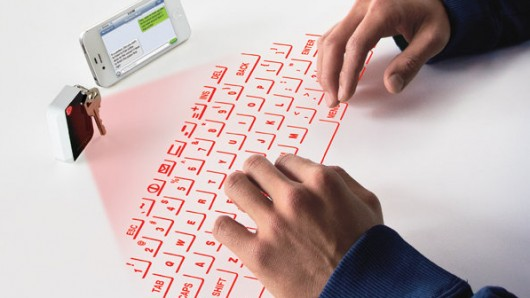
\includegraphics[width=\textwidth]{virtual-keyboard}
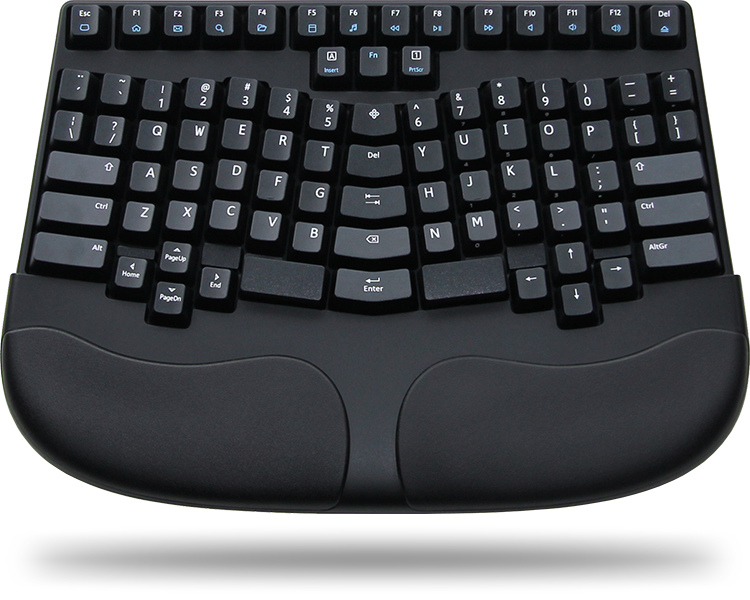
\includegraphics[width=\textwidth]{ergonomickeyboard}
\caption{Examples of keyboard devices}
\end{figure}

A keyboard is an indirect input device using an arrangement of buttons or keys, acting as mechanical levels or electronic switches. 
Common keyboards are typewriter style devices, with many buttons representing alphanumeric characters as well as a small number of additional function keys.
Desktop keyboards usually have from 100 to 105 keys, while laptop and other small device keyboards contain less.
All standard keyboards have a typing area used for letters of the alphabet, numbers, punctuation, and other basic characters.
However, there are also composite devices that have keyboard like features, such as video game controllers. 
Game controller buttons offer contextual and situational functionality depending on the application in use.
The keyboard is the best input device for writing, and takes advantage of the ease on text as a medium of communication between the user and the computer.
Problems are the lack of intuitive input methods for non text applications.
Many applications use a combination of function and character keys to perform actions in non-text-based applications, bringing a learning curve in order to use these applications effectively.

\subsection{Pointing Devices}
 A pointing device is a device that allows a user to input spacial data to a computer. 
 Many common input devices fall under this classification. 
 CAD systems and graphical user interfaces allow the user to control and provide data to the computer using physical motion.
 These movements are then echoed on the screen in some way, whether it be by an on-screen cursor, or some change in the visual output.
 Pointing devices are usually controlled by either physical movement of an object, or touching a surface.
 Examples of devices based on motion are the mouse, trackball, and joystick, and those based on touch are the graphics tablet, stylus, touchpad, and touch screen.
 
 \subsubsection{Mouse}
 A mouse is a small, hand-held device that is pushed over a flat, horizontal surface.
 Older mouses used a physical ball at the base of the device, combined with sensors to detect when the ball rotates.
 When the mouse moves and rotation is sensed, the distance and directional information is sent from the mouse to the computer.
 A more modern approach is the optical mouse, which uses infrared light instead of a roller to detect changes in position.
 
 \begin{figure}
 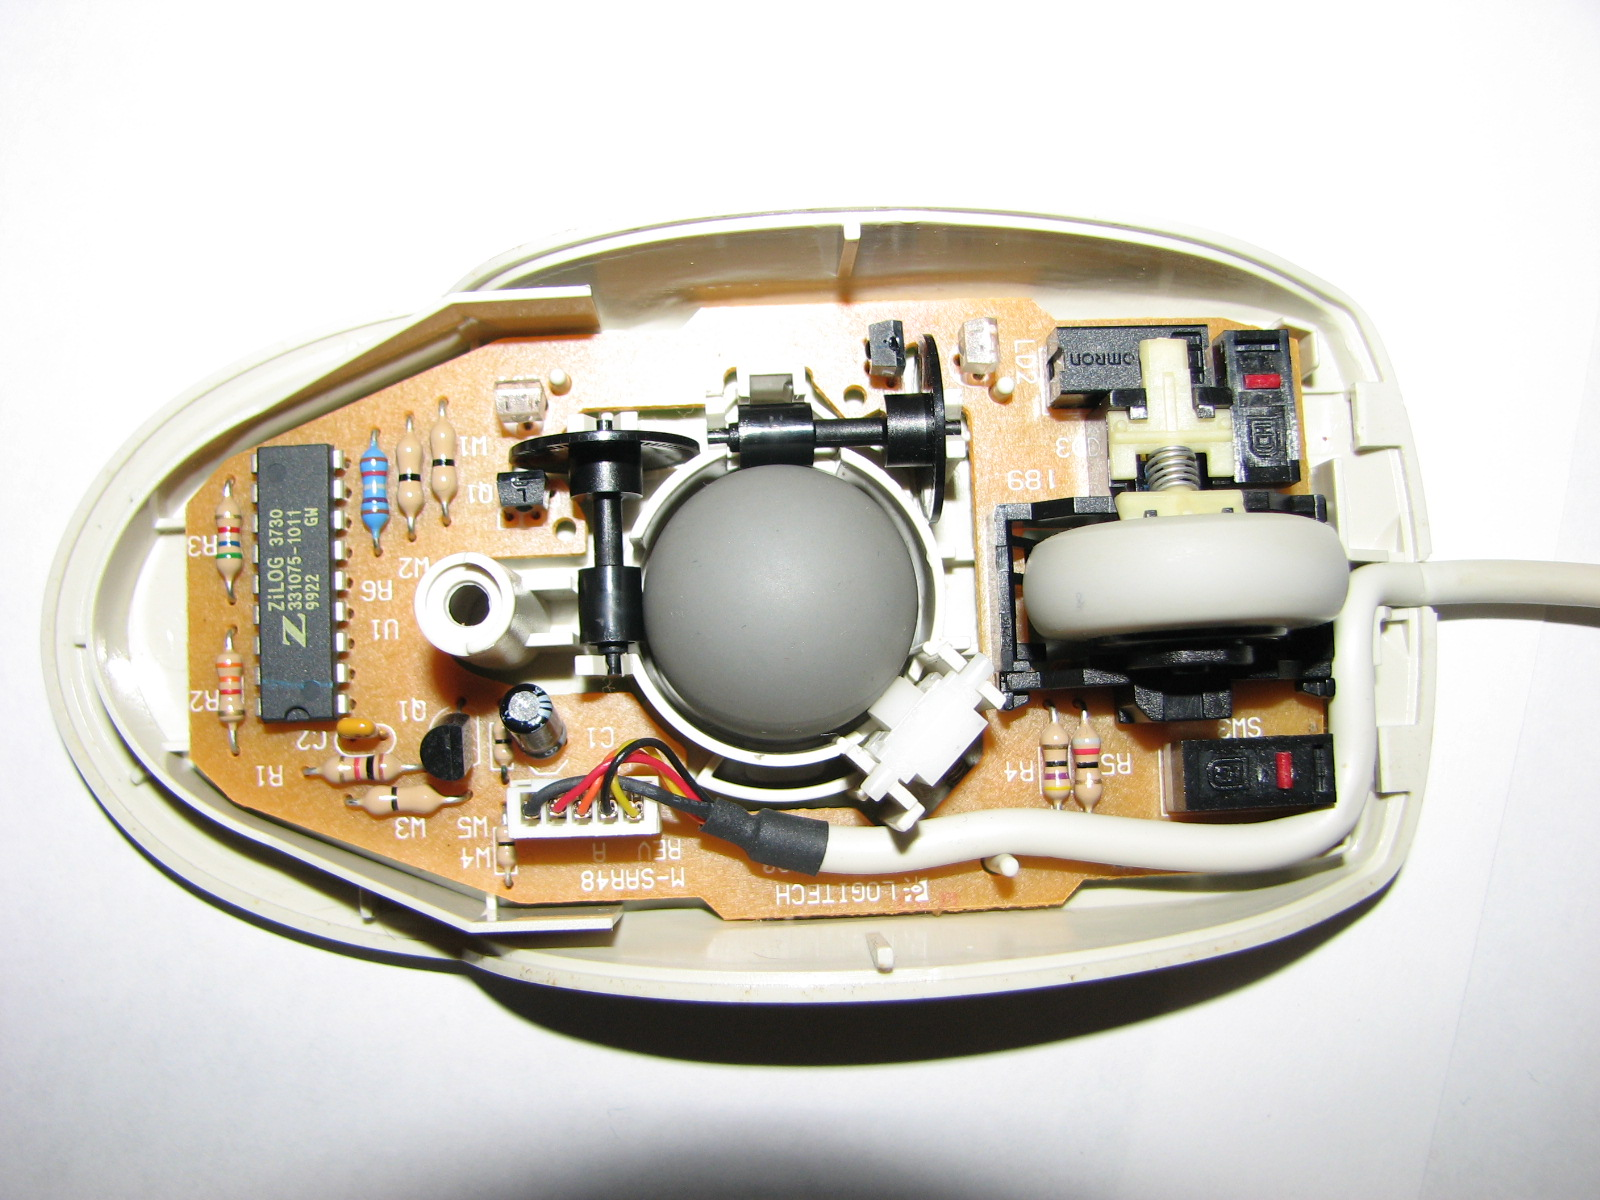
\includegraphics[width=0.5\textwidth]{mechmouse}
 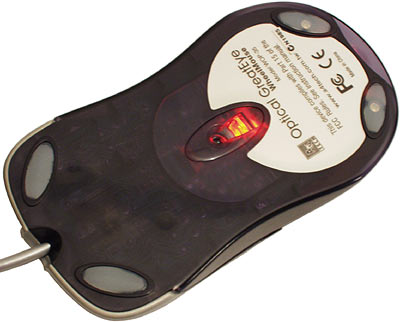
\includegraphics[width=0.5\textwidth]{opticalmouse}
 \caption{The two different types of mice. Left: mechanical mouse with a roller Right: An optical mouse}
 \end{figure}
 
 \begin{figure}
 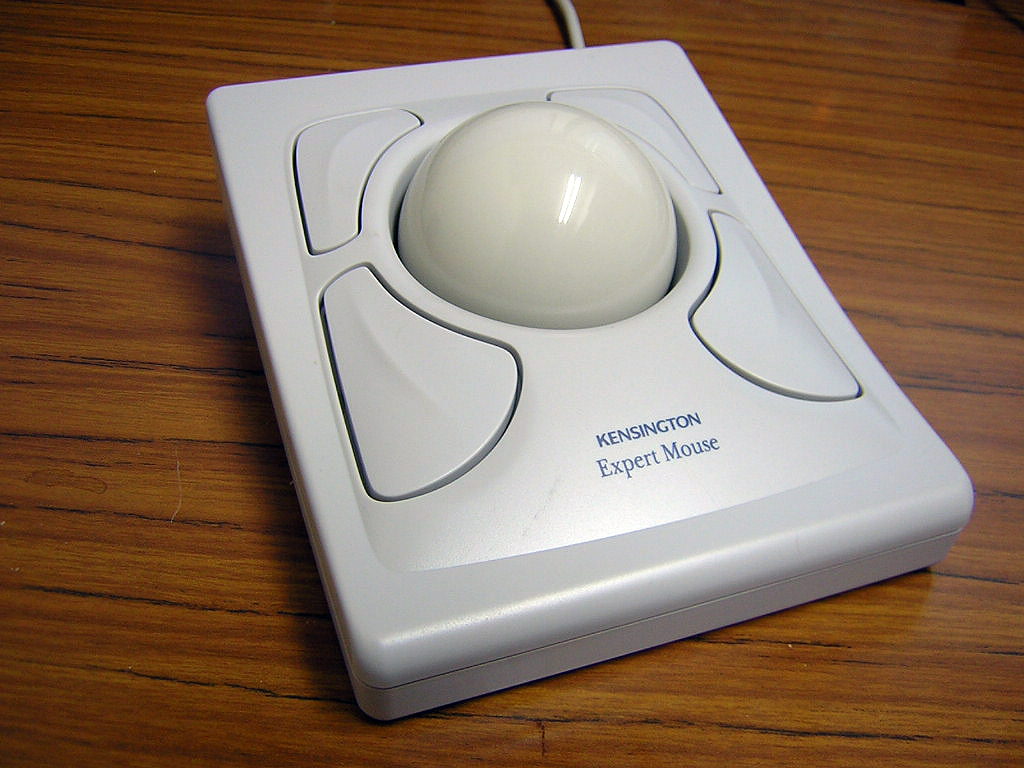
\includegraphics[width=0.9\textwidth]{trackball}
 \caption{A trackball}
 \end{figure}
 
 \subsubsection{Trackball}
 
 A trackball consists of a roller ball held by a socket containing sensors to detect rotation.
 It is essentially an upside-down mouse with an exposed ball.
 The trackball differentiates itself from the mouse by not having a limit on it's effective travel.
 Since a mouse requires the device to physically move, it is possible for the user to run out of workspace for the mouse to move on.
 When using the trackball, the user rotates the ball in place, so it does not run into this issue.
 Trackballs are commonly used for high precision applications, although there is no data on whether users are more accurate with trackballs compared to mice.
 
 \subsubsection{Joystick}
 
 A joystick is a handle stick that pivots on a base. 
 The user can freely change the stick's position by using constant force.
 The joystick reports it's angle or direction to the device it's controlling.
 Joysticks are commonly used to pilot aircrafts, and control video games. 
 
 
 \subsubsection{Touchpad}
 A touchpad or trackpad is a flat surface that can detect finger contact. 
 It is a stationary device, usually integrated into laptop computers. The trackpad controlled in a way similar to the mouse, where horizontal movement of the finger on the trackpad is converted into input. 
 Trackpads use a two layer grid of electrodes to detect movement: one layer for horizontal and one for vertical.
 
 \subsubsection{Tablet}
 A graphics or digitizing tablet is a special tablet that is similar to a touchpad. 
 However, it is controlled with a digital pen or stylus that is held and used like a normal pen.
 An alternative control device for tablets is called a puck. 
 This is a mouse like device that can detect absolute position and rotation.
 Professional pucks have a reticle which allows the user to see the exact point on the tablet's surface targeted by the puck, for detailed CAD work.
 Graphics tablets are commonly used to create 2D computer graphics, because their input similarities to traditional drawing techniques. 
 
 \subsubsection{Pen}
 
 As mentioned above, touch panels can be used with rigid styli to simulate the experience of writing. 
 However, the pen itself can also be digitized to capture additional information for various applications. 
 An active pen is an input device that includes electronic components and allows users to write directly onto the LCD screen surface of a computing device.
 The active pen's electronic components generate wireless signals that are picked up by a built-in digitizer and transmitted to its dedicated controller, providing data on pen location, pressure and other functionalities. 
 Additional features enabled by the active pen's electronics include palm rejection to prevent unintended touch inputs, and hover, which allows the computer to track the pen's location when it is held near, but not touching the screen. 
 Most active pens feature one or more function buttons (e.g. eraser and right-click) that can be used in place of a mouse or keyboard.

\subsection{Touch Screen Devices}

A touch screen is an input device layered on top of a display. 
Users provide input by touching the screen with one or more fingers, or with a special stylus/pen.
This method of input allows users to directly interact with what is displayed, as opposed to using an indirect input device such as a mouse or touchpad.

One major advantage touch screens offer over other input devices is ease of use.
While frequent computer users are familiar with using a mouse and keyboard, touching icons on a screen is intuitive even for those with limited to no computer experience.
This ease of use can reduce the learning curve and increase productivity when using user interfaces.
Touchscreens are also faster to use than traditional input methods.
When a user interacts with a computer using a mouse and keyboard, there are many small adjustments the user needs to make; they need to locate the pointer, and adjust for the mouse acceleration.
Direct interaction allows for users to interact with the computer without worrying about correlating the interaction space to the virtual space. 

There are many ways to build a touch screen.
The key points in any implementation are to recognize one or more fingers touching a display, to interpret the command these touches represent, and to communicate with an application.
In the most popular implementations, capacitive and resistive sensing, touch screens are comprised of four layers:

\begin{itemize}
\item Top polyester coated with a transparent metallic conductive coating on the bottom
\item Adhesive spacer
\item Glass layer coated with a transparent metallic conductive coating on the top
\item Adhesive layer on the backside of the glass for mounting
\end{itemize}

\subsubsection{Resistive Sensing}
Resistive touch panels are composed of two thin, flexible sheets coated with a resistive material and separated by a small gap.
The position on screen contacted by a finger, stylus, or other object is detected using changes in pressure. 
The monitor features a simple internal structure: a glass screen and a film screen separated by a narrow gap, each with a transparent electrode film (electrode layer) attached. 
Pressing the surface of the screen presses the electrodes in the film and the glass to come into contact, resulting in the flow of electrical current. 
The point of contact is identified by detecting this change in voltage.

\begin{center}
\begin{figure}
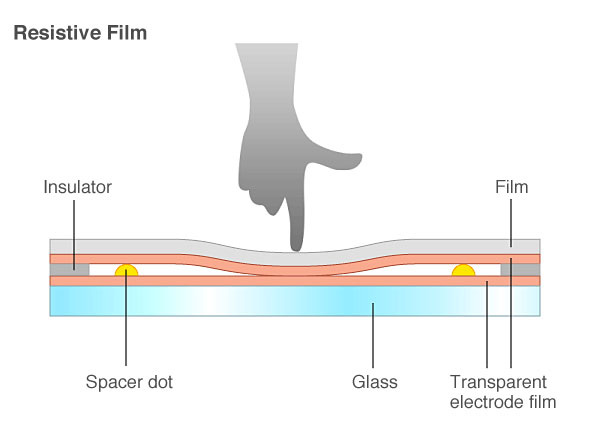
\includegraphics[width=0.9\textwidth]{resistive}
\caption{A resistive sensor}
\end{figure}
\end{center}

Resistive technology is low cost due to the simple structure of the touch screen and controller circuit.
Analog senors have high resolution, the most common being 4096 by 4096 dots-per-inch (DPI), as well as high accuracy, while consuming low amounts of power during operation.
Resistive touch screens can be used with any object, since the system only requires contact. 
This allows for users to use pens and gloves to interact with a device.
Disadvantages include it's poor responsiveness compared to other developed sensing methods, generally working with harder presses, lower light transmittance causing a reduction in screen quality, and a decrease in accuracy in screen sizes about 24 inches.
While high resolutions would allow for more accurate and more detailed sketching, the poor responsiveness would make resistive panels a poor substitute for traditional drawing media.

 




\subsubsection{Capacitive Sensing}
Capacitive touch panels use the natural flow of electricity through the human body, also called body capacitance, as an input device.
They are most commonly used consumer level hardware; seen in smart phones, tablets, and LCD monitors.
They are constructed from a wide variety of materials, such as copper, Indium tin oxide (ITO), and printed ink.
There are two types of capacitive technology; surface capacitive and projected capacitive.
Surface capacitive is is used in ATMs and on factory lines, but are growing more limited in application.
Projected capacitive was first designed and implemented for smart phones, and due to it's success has been growing in use.

 
\begin{center}
\begin{figure}
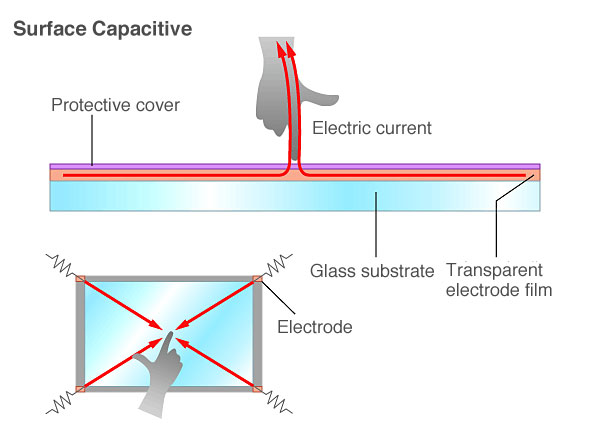
\includegraphics[width=0.9\textwidth]{surcap}
\caption{A surface capacitive sensor}
\end{figure}
\end{center}

\paragraph{Surface Capacitive Sensing}

is often used for larger sized displays (over 14 inches) that are used by the general public.
This accentuates their high durability and high screen quality.
Surface capacitive displays can be seen on ATM machines, ticket kiosks, arcade games, automation devices in factories and offices, and in the medical industry.

A surface capacitive panel is constructed using a glass sheet. 
A transparent conductive coating is placed over the sheet, and a glass protective coating is placed above that. 
Electrodes are placed on the four corners of the panel. 

The same phase voltage is imposed to the electrodes on the four corners, then a uniform electric field will be forming over the panel. 
When a finger touches on the panel, electrical current will flow from the four corners through the finger. 
Ratio of the electrical current flowing from the four corners will be measured to detect the touched point. 
The measured current value will be inversely proportional to the distance between the touched point and the four corners.

A surface capacitive touch panel has a simpler structure than a projected touch panel.
This allows for lower cost in production, high durability, and high visibility due to the main structure being a single glass layer. 
However, it's simplistic structure also means it is structurally difficult to detect two or more contact points simultaneously.
Surface capacitive can only detect bare finger touches, although some may detect touches through a thin pair of gloves.
Some surface capacitive displays support pen writing, but not simultaneous pen and touch.

\subsubsection{Surface Acoustic Wave (SAW) Sensing}

Surface acoustic wave (SAW) touch panels were developed mainly to address the drawbacks of low light transmittance in resistive film touch panels; to achieve bright touch panels with high levels of visibility. 
These are also called surface wave or acoustic wave touch panels. 
Aside from standalone LCD monitors, these are widely used in public spaces, in devices like point-of-sale terminals, ATMs, and electronic kiosks.

These panels detect the screen position where contact occurs with a finger or other object using the attenuation in ultrasound elastic waves on the surface. 
The internal structure of these panels is designed so that multiple piezoelectric transducers arranged in the corners of a glass substrate transmit ultrasound surface elastic waves as vibrations in the panel surface, which are received by transducers installed opposite the transmitting ones. 
When the screen is touched, ultrasound waves are absorbed and attenuated by the finger or other object. 
The location is identified by detecting these changes.

\begin{center}
\begin{figure}
\includegraphics[width=0.9\textwidth]{saw}
\caption{A surface acoustic wave sensor}
\end{figure}
\end{center}

The strengths of this type of touch panel include high light transmittance and superior visibility, since the structure requires no film or transparent electrodes on the screen. 
Additionally, the surface glass provides better durability and scratch resistance than a capacitive touch panel. 
Another advantage is that even if the surface does somehow become scratched, the panel remains sensitive to touch. 
On a capacitive touch panel, surface scratches can sometimes interrupt signals. 
Structurally, this type of panel ensures high stability and long service life, free of changes over time or deviations in position.
Weak points include compatibility with only fingers and soft objects (such as gloves) that absorb ultrasound surface elastic waves. 
These panels require special-purpose styluses and may react to substances like water drops or small insects on the panel.

\paragraph{Projected Capacitive Sensing}

is often used for smaller screen sizes than surface capacitive touch panels. 
They've attracted significant attention in mobile devices. 
The iPhone, iPod Touch, and iPad use this method to achieve high-precision multi-touch functionality and high response speed.
However, they have also seen use in other areas of display technology, with Microsoft's Surface Hub implementing a 55-inch projected capacitive display.

The internal structure of these touch panels consists of a substrate incorporating an IC chip for processing computations, over which is a layer of numerous transparent electrodes is positioned in specific patterns. 
The surface is covered with an insulating glass or plastic cover. 
When a finger approaches the surface, electrostatic capacity among multiple electrodes changes simultaneously, and the position were contact occurs can be identified precisely by measuring the ratios between these electrical currents.

\begin{figure}
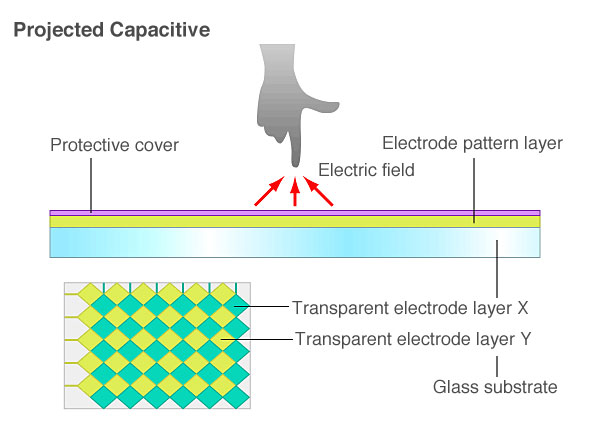
\includegraphics[width=0.9\textwidth]{projcap}
\caption{A projected capacitive sensor}
\end{figure}

A unique characteristic of a projected capacitive touch panel is the fact that the large number of electrodes enables accurate detection of contact at multiple points (multi-touch). 
However, the projected capacitive touch panels featuring indium-tin-oxide (ITO) found in smart phones and similar devices are poorly suited for use in large screens, since increased screen size results in increased resistance (i.e., slower transmission of electrical current), increasing the amount of error and noise in detecting the points touched.
Larger touch panels use center-wire projected capacitive touch panels in which very thin electrical wires are laid out in a grid as a transparent electrode layer.
 
While lower resistance makes center-wire projected capacitive touch panels highly sensitive, they are less suited to mass production than ITO etching.
Unlike resistive film touch panels, they do not respond to touch by clothing or standard styli.
They feature strong resistance to dust and water drops and high durability and scratch resistance. 
In addition, their light transmittance is higher, as compared to resistive film touch panels allowing for higher quality displays.



\subsubsection{Summary of Touch Panel Technology}

\begin{center}
\begin{tabular}{| p{5cm} | l | p{4cm} | l |}
\hline
\textbf{Method} & \textbf{Resistive} & \textbf{Capacitive} & \textbf{SAW} \\ \hline
\textbf{Light Transmittance} & Poor & Good & Good \\ \hline
\textbf{Finger Touch} & Excellent & Excellent & Excellent \\ \hline
\textbf{Gloved Touch} & Excellent & None & Good \\ \hline
\textbf{Stylus Touch} & Excellent & Poor (Special purpose devices) & Good \\ \hline
\textbf{Maximum Single User Touch Points} & One & Ten & Two \\ \hline
\textbf{Accuracy} & Excellent & Good & Good \\ \hline
\textbf{Durability} & Poor & Excellent & Excellent \\ \hline
\textbf{Water Resistance} & Excellent & Excellent & Poor \\ \hline
\textbf{Cost} & Reasonable & Not reasonable & Not reasonable \\ \hline
\end{tabular}
\end{center}

\section{Advanced User Interaction: Input using Gesture}

A gesture is a form of communication where visible body action communicate particular messages.
Common gestures are performed by hand and arm movements.
Other forms of physical non-verbal communication, such as purely expressive display, proxemics, and joint attention differ from gestures, which communicate specific messages.
While some gestures are ubiquitous, such as pointing, which differs little in intent from one place to another, many do not have universal meanings and are defined differently in different cultures.

\subsection{Types of Gestures}

Morris (1978) describes two main types of gestures: primary and incidental.

Primary gestures are voluntary movements that a person uses with intent of communicating a message. There are three main types:

\begin{enumerate}
\item Emblems: These are gestures that have a direct verbal equivalent. 
For example, a waving of a hand upon an encounter means hello. 
Emblems tend to form in situations where speech is challenging or impossible.
Airport controllers on runways communicate with gestures because the planes make it impossible to hear.

\item Illustrators: These gestures are closely linked with speech, and serve to clarify, or add to the content of the message. 
Illustrators are made by hand movements.
A common example of an illustrator is pointing.

\item Reinforcers: There are gestures that help regulate the flow of conversation.
For example, a head nod during conversation means that the current speaker should continue, or an upwards point might mean to wait to continue speaking.
\end{enumerate}

Secondary, or incidental gestures are unintentional, but despite their lack of direct message are still important in conversation.
Gestures such as grooming the hair, fidgeting, looking down or away, or looking at a clock are all examples of involuntary gestures.
While they do not directly communicate, secondary gestures can still send information about the current state of their user.
This is called leakage, when true feelings or attitudes are revealed despite what the overt signals are communicating.
For example, a man in a rush might say, "Yeah, I can talk" while looking at a watch.
Secondary gestures are not as important for Human Computer Interaction, however care must be taken so involuntary gestures do not accidentally get inputted. 

Human computer interaction further distinguishes between types of gestures,; splitting them into two major categories.

\begin{enumerate}

\item Offline: These gestures are processed after the user interaction with the object. For example, drawing a circle activates a menu.

\item Online: These gestures directly manipulate an object. A common example is taking two fingers and spreading them while touching an object to zoom in on the object.
\end{enumerate} 



\subsection{Multi Touch Gestures}

Multi-touch gestures are predefined motions used to interact with multi-touch devices.
Many modern consumer electronics like smartphones, tablets, laptops, or desktop computers feature functions triggered by multi-touch gestures.
They tend to be direct input methods with simple to understand functionality heavily based on the gesture used, allowing non-technical people to quickly configure and navigate multi-touch applications.

Common multi-touch gestures are:

\subsubsection{Tap}

\begin{figure}
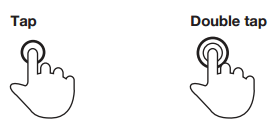
\includegraphics[width=\textwidth]{Taps}
\end{figure}

Taps are performed by briefly touching a screen with a fingertip. 
Most systems differentiate between single and double taps, preformed by tapping the screen once or twice respectively.
Taps are generally used for selecting items, with single and double taps offering different types of selection.
Taps are both online and offline gestures, since the number of taps need to be processed, but directly interact with objects being tapped.

\subsubsection{Drag}

\begin{figure}
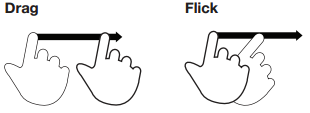
\includegraphics[width=\textwidth]{Drags}
\end{figure}

Drags are performed by moving a fingertip over a surface without losing contact. 
An alternative type of drag is the flick, which is performed by the same method as the drag, only faster.
Drags are generally used to move elements, making them online gestures.

\subsubsection{Pinch and Spread}

\begin{figure}
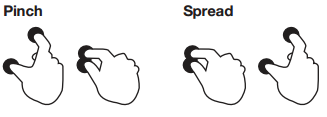
\includegraphics[width=\textwidth]{Pinch}
\end{figure}

Pinches are preformed by taking any number of fingertips and enclosing them towards a point. spread gestures are the inverse action. Generally these online gestures are used for magnification.

\subsubsection{Rotate}

\begin{figure}
\includegraphics[width=\textwidth]{Rotate}
\end{figure}

Rotate gestures are performed by moving two or more fingertips in a circular pattern around a point. The rotation point is used as the input location.
Rotation is an online gesture.

\subsubsection{Press}

\begin{figure}
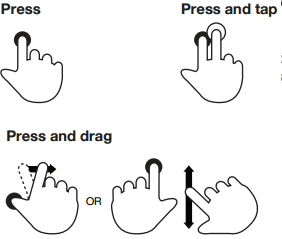
\includegraphics[width=\textwidth]{Presses}
\end{figure}

Presses are performed by touching a screen for an extended period of time. 
Presses can be combined with other touch gestures to allow for a deeper level of user interaction.
Presses are offline gestures, since the duration of the press must be processed, and usually results in context menus used for enhancing information about the object.



\subsection{Pen Gestures}

Pen gestures recognize certain shapes as not handwriting, but as an indicator of a special command.
For example, a pig-tail shape (used often as a proofreader's mark) would indicate a delete operation. 
Depending on the implementation, what is deleted might be the object or text where the mark was made, or the stylus can be used as a pointing device to select what it is that should be deleted.
These types of gestures are offline.

Pens can be used to perform many of the multi-touch gestures, but the pen is just treated as a finger in these scenarios.

\begin{figure}
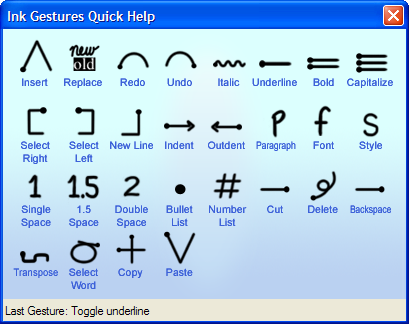
\includegraphics[width=\textwidth]{pen-gestures}
\caption{Examples of pen gestures in InkGesture by Jumping Minds}
\end{figure}

\subsection{Three Dimensional Gesture Recognition}

While older forms of gesture recognition attempt to translate physical interaction with an input device in oder to form gesture based commands, more modern approaches attempt to do away with the intermediary and directly interpret motions of the human body.
This is accomplished using computer vision techniques, as well as different types of cameras used to capture and understand a three dimensional environment.
The two types of cameras used for this are depth aware cameras and stereo cameras.

Depth aware cameras are capable of generating a depth map, an image representing the physical distance between captured objects and the camera.
These cameras use structured light or time-of-flight techniques to capture this information.
Current depth aware cameras are capable of capturing and representing a scene accurately between 1 to 15 feet with error in the millimeters.

Stereo cameras use two cameras whose relations to one another are known. 
Using information such as the distance between the two cameras, the focus points, and the lens information, a three dimensional representation of the captures scene can be approximated. 
Infrared emitters are commonly used to get this information.
In combination with direct motion measurement, gestures can be directly detected.

Once this information is captured a variety of techniques can be used to analyze the scene and detect gestural information

\subsubsection{3-D Model Analysis}

A 3-D model can be constructed from the depth data and analyzed for forms approximating common gestures. 
This method is very computationally intensive, and is currently not used for real time applications.
However, it might be possible to map simple primitives, such as a sphere for the palm of the hand and and cylinders for the fingers, in oder to speed up this process.

\subsubsection{Skeletal Analysis}

Instead of using a complicated model, only joint angle parameters and segment length analysis is used to approximate a simple skeletal structure. By only analyzing key parameters, skeletal analysis allows for much faster speeds compared to a full model analysis.
The simple structure can also be matched to a pattern database using machine learning techniques in order to further increase speeds.

\subsubsection{Appearance-based Analysis}

These models don’t use a spatial representation of the body, because they derive the parameters directly from the images or videos using a template database. 
Some are based on the deformable 2D templates of the human parts of the body, particularly hands.
Deformable templates are sets of points on the outline of an object, used as interpolation nodes for the object’s outline approximation. 
One of the simplest interpolation function is linear, which performs an average shape from point sets, point variability parameters and external deformators. 
These template-based models are mostly used for hand-tracking, but could also be of use for simple gesture classification.



\end{document}